\section{Technische Lösung}

    Als Lösung dient eine Künstliche Intelligenz, die die Fehlerursache vollautomatisch eingrenzt. Dadurch muss sich das Instandhaltungspersonal nicht mehr mühsam durch komplizierte Log-Dateien kämpfen, sondern kann die Anlage schnellstmöglich wieder in den produktiven Zustand überführen. Die eigentliche Herausforderung besteht nun darin, dieses Konzept in funktionierenden Code zu übersetzen. Das folgende Konzept beschreibt hierfür einen möglichen Lösungsansatz.


    \subsection{Technisches Lösungskonzept}
    Das Lösungskonzept ist in Abbildung~\ref{fig:fehlersupport_ablauf} dargestellt und gliedert sich in zwei grundlegende Phasen: 
    
    Eine kontinuierliche Informationserfassungsphase während des laufenden Anlagenbetriebs. Diese sind in der Grafik im oberen Kästchen dargestellt sowie eine Analysephase, die ausschließlich im Fehlerfall aktiviert wird. Diese ist im unteren Teil der Grafik dargestellt. 

        \begin{figure}[H]
        \centering
        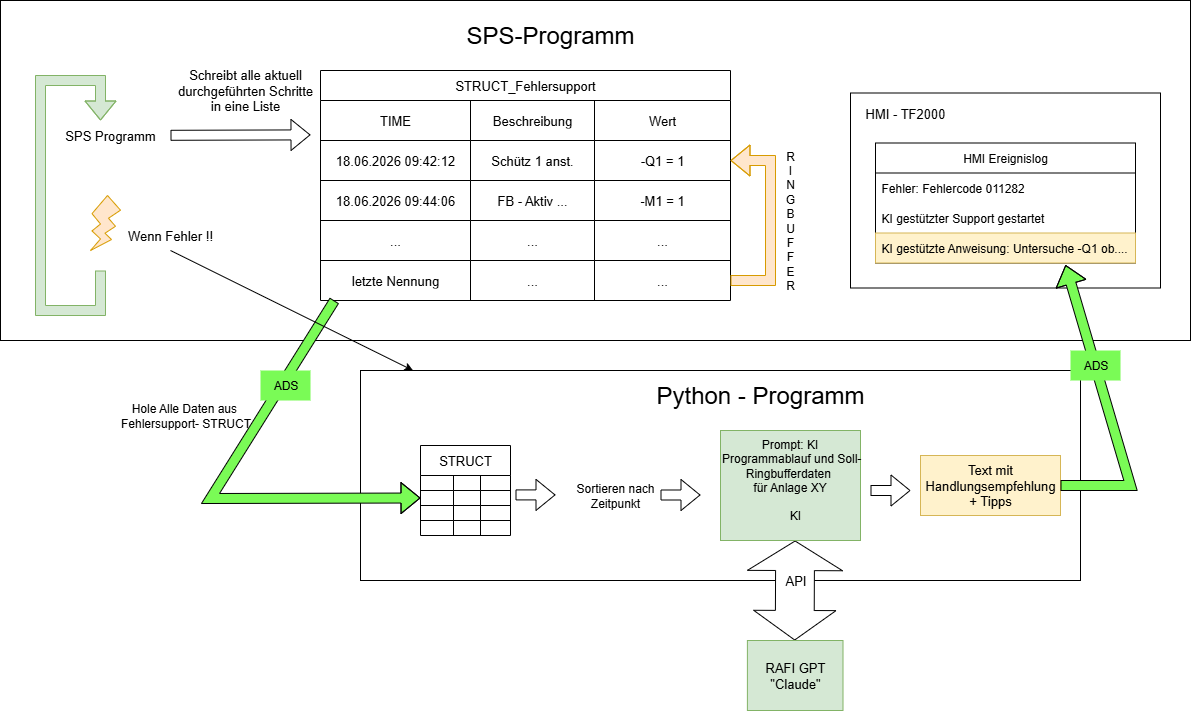
\includegraphics[width=\textwidth]{images/UmsetzungIntelligenterFehlersupport.drawio.png}
        \caption{Programmstruktur Intelligenter Fehlersupport}
        \label{fig:fehlersupport_ablauf}
        \end{figure}


    \subsubsection{Kontinuierliche Erfassung im Normalbetrieb}

        Im regulären Anlagenbetrieb werden Bedienereignisse, Anlagenzustände sowie Fehler- und Wartungseinträge fortlaufend in eine gemeinsame Ringpuffer-Datenstruktur als Array innerhalb des SPS-Programms geschrieben. Ein solcher Ringpuffer ist eine Datenspeicherstruktur, bei der nach Erreichen der letzten freien Speicherstelle der jeweils älteste Eintrag automatisch durch das neueste Element überschrieben wird. Das zugrundeliegende Prinzip ist in Abbildung~\ref{fig:ringbuffer} dargestellt.

        % Bild Ringbuffer
        \begin{figure}[H]
            \centering
            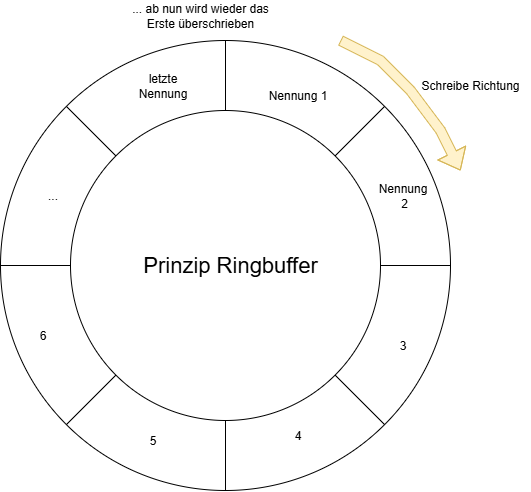
\includegraphics[width=\imgmedium]{images/RINGBUFFER.drawio.png}
            \caption{Prinzip des Ringpuffers}
            \label{fig:ringbuffer}
        \end{figure}

        Dadurch entsteht ein rollierender Datensatz der letzten Anlagenereignisse, in dem stets die zeitlich neuesten Vorgänge vorgehalten werden.
        
        Die Inhalte, die an bestimmten Programmstellen gespeichert werden sollen, sind dabei flexibel wählbar. Es wird jedoch empfohlen, alle aktorischen Elemente der Anlage durch aussagekräftige Beschreibungen zu erfassen. Auf diese Weise kann das System präzise angeben, welche Zylinder zu einem bestimmten Zeitpunkt beispielsweise ausgefahren sein müssten. Im Fehlerfall sieht das Personal sofort, ob diese Soll-Bedingung, also ob der Zylinder ausgefahren ist, erfüllt ist, wodurch sich die Fehlerursache schnell und zielgerichtet bestimmen lässt.

        Ebenso sollten regelmäßig aktive Programmschritte in den Speicher geschrieben werden, um bei Ablaufproblemen exakt nachvollziehen zu können, in welchem Produktionsschritt sich die Anlage gerade befindet. Darüber hinaus empfiehlt sich die Protokollierung verschiedener externer Einflüsse, wie etwa der zuvor genannten Ober- und Untergrenzen für den aktiven Druck im Pneumatiksystem. Ebenso sollten Bedienerinteraktionen erfasst werden, sprich gedrückter Knöpfe oder sonstiger Eingaben.

        Solange kein Fehler vorliegt, werden all diese Einträge fortlaufend durch neuere Daten überschrieben. Da sich die Anlage im produktiven Zustand befindet, ist dieser Datenverlust unkritisch, da kein Analysebedarf besteht. Spannend wird es hingegen, sobald die Anlage in einen Fehlerzustand wechselt.
    
    \subsubsection{Fehlerausgelöste Analysephase}

        Tritt an der Anlage ein Fehler auf, wird anlagenintern ein Fehlerbit gesetzt, auf das ein Mikrocomputer über OPC-UA reagieren kann. Auf diesem Mikrocomputer läuft ein Python-Skript, welches im ausgelösten Fall nacheinander die folgenden Schritte ausführt:

        \textbf{2.1 Auslesen der aktuellen Ringbufferinhalte:}

        Zunächst wird der vollständige Inhalt des Ringpuffers unmittelbar nach Auslösen des Fehlers aus der SPS-Steuerung über OPC-UA ausgelesen und an den Computer übermittelt.


        \textbf{2.2 Zeitliche Sortierung der Daten:}

        Im nächsten Schritt werden die ausgelesenen Daten im Python-Programm anhand ihrer Zeitstempel in eine chronologisch korrekte Reihenfolge gebracht. Dies ist notwendig, da aufgrund des Ringpufferprinzips zunächst keine lineare zeitliche Ordnung in den Rohdaten vorliegt. Mithilfe der Zeitstempel lässt sich diese Sortierung in Python jedoch problemlos umsetzen.

        \textbf{2.3 KI gestütztes Eingrenzen des Fehlers:}

        Das Python-Programm übermittelt die chronologisch sortierten Ereignisdaten per API an eine KI-Cloud. Entscheidend für die Qualität der anschließenden Auswertung ist ein präziser, vordefinierter System-Prompt, der dem KI-Modell den spezifischen Maschinenkontext vermittelt. Erst durch diese kontextuelle Grundlage ist das KI-System in der Lage, komplexe Zusammenhänge zwischen den verschiedenen Ereignissen zu erkennen und eine fundierte Einschätzung zur Fehlerursache zu formulieren. Darüber hinaus weist der System-Prompt die KI an, die ermittelte Ursache kompakt und verständlich in wenigen Sätzen für das Instandhaltungspersonal zusammenzufassen.

        \textbf{2.4 Darstellen der KI-Ergebnisse auf dem HMI-Display der Anlage:}

        Die Ausgabe des KI-Systems wird im Anschluss über die OPC-UA-Schnittstelle an das HMI übermittelt und dort in einem übersichtlichen Textfeld dargestellt. Die von der KI verfassten Sätze liefern dem Instandhaltungspersonal eine präzise Fehlerursache, eine entsprechende Eingrenzung sowie eine konkrete Handlungsempfehlung. Durch die direkte Visualisierung auf dem HMI-Display sind diese wertvollen Informationen für den Werker sofort abrufbar und im direkten Arbeitsumfeld anwendbar.